\documentclass[10pt]{beamer}
\usepackage[utf8]{inputenc}
\usepackage{tikz, pgfplots}
\pgfplotsset{compat=1.18}
\usetikzlibrary{positioning}
\usetikzlibrary{trees}
\usetikzlibrary{shapes.geometric, arrows.meta, positioning}
\usepackage{xcolor}
\usepackage{graphicx}
\usepackage{subcaption}
\usepackage{hyperref} 
\usepackage{colortbl} % Required for \rowcolor
\usepackage{animate}
\usepackage[T1]{fontenc}
\usepackage{amsmath, amsfonts, amssymb}
\usepackage{cancel}
\usepackage[french]{babel}
\usepackage[normalem]{ulem}

% Theme và màu sắc cho beamer
\usetheme{AnnArbor}
\usecolortheme{seahorse}

% Định nghĩa và thiết lập màu sắc chung
\definecolor{mydarkblue}{RGB}{0,51,102}
\setbeamercolor{structure}{fg=mydarkblue}
\setbeamercolor{frametitle}{bg=mydarkblue, fg=white}
\setbeamercolor{title}{fg=mydarkblue}
\setbeamercolor{item}{fg=mydarkblue}
\setbeamercolor{block title}{bg=mydarkblue, fg=white}
\setbeamercolor{block body}{bg=white, fg=black}
\setbeamercolor{section in toc}{fg=mydarkblue}
\setbeamercolor{subsection in toc}{fg=mydarkblue}
\setbeamercolor{caption name}{fg=mydarkblue}
\setbeamercolor{author}{fg=mydarkblue}
\setbeamercolor{date}{fg=mydarkblue}
\setbeamercolor{institute}{fg=mydarkblue}
\setbeamertemplate{caption}[numbered]
\usepackage{multirow}
\title{Rapport Hebdo}
\author{Viet Anh Quach}
\institute{3SR}
\date{\today}

\begin{document}

\begin{frame}
    \titlepage
\end{frame}


\section{DEM}

% 03102025
\begin{frame}{Non-linéaire critère de Coulomb au pic des échantillons denses}
    \begin{columns}
        \begin{column}{0.5\textwidth}
            \begin{figure}[h]
                \centering
                \scalebox{0.08}{\includegraphics{Nonlinear_Dense.png}}
                \caption{Non-linéaire critère de Coulomb au pic des échantillons denses}
            \end{figure}
        \end{column}
        \begin{column}{0.5\textwidth}
            \begin{figure}[h]
                \centering
                \scalebox{0.2}{\includegraphics{angleFrictionInterne.png}}
                \caption{Non-linéaire critère de Coulomb au pic des échantillons denses}
            \end{figure}
        \end{column}
    \end{columns}
                Aucun explication: Ponce and Bell,1971, Stroud, 1971; Shinji Fukushima 1984;
Papier: M. Vivoda Prodan et al, 2024 ;
Daosheng Ling et al 2024;
ASCE...
\end{frame}


\begin{frame}{Modifications sur les paramètres d'un échantillon lâche}
    kineticStress = 1: Ajouter les parties:
    \begin{align*}
    \dot{r} &= h\dot{s} + \cancel{\dot{h}s} \\
    \ddot{s} &= h^{-1}(\ddot{r} - 2\dot{h}\dot{s} - \cancel{\ddot{h}s})
    \end{align*}
    Échantillon lâche: $ \mu_{\text{isoComp}} = \mu_{\text{triaxialComp}} = 0.5$ \\
    Réglage sur Kappa:
    \begin{align*}
            W_{particule} = K / (K + 1) = 1 / (1 + 1) = 0.5; \\
            k_n^{elas} = k_n \times W_{particule} \times \eta_{amort}; \\
            \sigma_3 = 30 \times 10^3; \\
    \kappa = \dfrac{k_n^{elas}}{\sigma_3 \overline{a}} = \dfrac{3\times10^{6}/2}{30\times10^{3} \times (2 \times 0.004)} = 6250
\end{align*}

\end{frame}



\begin{frame}{Influnce du terme dynamique}
    \begin{columns}
        \begin{column}{0.5\textwidth}
            \begin{figure}
                \centering
                \scalebox{0.5}{\input{KineticComp.tex}}
                \caption{kineticStress = 1}
            \end{figure}
        \end{column}
        \begin{column}{0.5\textwidth}
            \begin{figure}
                \centering
                \scalebox{0.5}{% GNUPLOT: LaTeX picture with Postscript
\begingroup
  \makeatletter
  \providecommand\color[2][]{%
    \GenericError{(gnuplot) \space\space\space\@spaces}{%
      Package color not loaded in conjunction with
      terminal option `colourtext'%
    }{See the gnuplot documentation for explanation.%
    }{Either use 'blacktext' in gnuplot or load the package
      color.sty in LaTeX.}%
    \renewcommand\color[2][]{}%
  }%
  \providecommand\includegraphics[2][]{%
    \GenericError{(gnuplot) \space\space\space\@spaces}{%
      Package graphicx or graphics not loaded%
    }{See the gnuplot documentation for explanation.%
    }{The gnuplot epslatex terminal needs graphicx.sty or graphics.sty.}%
    \renewcommand\includegraphics[2][]{}%
  }%
  \providecommand\rotatebox[2]{#2}%
  \@ifundefined{ifGPcolor}{%
    \newif\ifGPcolor
    \GPcolortrue
  }{}%
  \@ifundefined{ifGPblacktext}{%
    \newif\ifGPblacktext
    \GPblacktextfalse
  }{}%
  % define a \g@addto@macro without @ in the name:
  \let\gplgaddtomacro\g@addto@macro
  % define empty templates for all commands taking text:
  \gdef\gplbacktext{}%
  \gdef\gplfronttext{}%
  \makeatother
  \ifGPblacktext
    % no textcolor at all
    \def\colorrgb#1{}%
    \def\colorgray#1{}%
  \else
    % gray or color?
    \ifGPcolor
      \def\colorrgb#1{\color[rgb]{#1}}%
      \def\colorgray#1{\color[gray]{#1}}%
      \expandafter\def\csname LTw\endcsname{\color{white}}%
      \expandafter\def\csname LTb\endcsname{\color{black}}%
      \expandafter\def\csname LTa\endcsname{\color{black}}%
      \expandafter\def\csname LT0\endcsname{\color[rgb]{1,0,0}}%
      \expandafter\def\csname LT1\endcsname{\color[rgb]{0,1,0}}%
      \expandafter\def\csname LT2\endcsname{\color[rgb]{0,0,1}}%
      \expandafter\def\csname LT3\endcsname{\color[rgb]{1,0,1}}%
      \expandafter\def\csname LT4\endcsname{\color[rgb]{0,1,1}}%
      \expandafter\def\csname LT5\endcsname{\color[rgb]{1,1,0}}%
      \expandafter\def\csname LT6\endcsname{\color[rgb]{0,0,0}}%
      \expandafter\def\csname LT7\endcsname{\color[rgb]{1,0.3,0}}%
      \expandafter\def\csname LT8\endcsname{\color[rgb]{0.5,0.5,0.5}}%
    \else
      % gray
      \def\colorrgb#1{\color{black}}%
      \def\colorgray#1{\color[gray]{#1}}%
      \expandafter\def\csname LTw\endcsname{\color{white}}%
      \expandafter\def\csname LTb\endcsname{\color{black}}%
      \expandafter\def\csname LTa\endcsname{\color{black}}%
      \expandafter\def\csname LT0\endcsname{\color{black}}%
      \expandafter\def\csname LT1\endcsname{\color{black}}%
      \expandafter\def\csname LT2\endcsname{\color{black}}%
      \expandafter\def\csname LT3\endcsname{\color{black}}%
      \expandafter\def\csname LT4\endcsname{\color{black}}%
      \expandafter\def\csname LT5\endcsname{\color{black}}%
      \expandafter\def\csname LT6\endcsname{\color{black}}%
      \expandafter\def\csname LT7\endcsname{\color{black}}%
      \expandafter\def\csname LT8\endcsname{\color{black}}%
    \fi
  \fi
    \setlength{\unitlength}{0.0500bp}%
    \ifx\gptboxheight\undefined%
      \newlength{\gptboxheight}%
      \newlength{\gptboxwidth}%
      \newsavebox{\gptboxtext}%
    \fi%
    \setlength{\fboxrule}{0.5pt}%
    \setlength{\fboxsep}{1pt}%
    \definecolor{tbcol}{rgb}{1,1,1}%
\begin{picture}(7200.00,5040.00)%
    \gplgaddtomacro\gplbacktext{%
      \csname LTb\endcsname%%
      \put(814,1144){\makebox(0,0)[r]{\strut{}$0$}}%
      \csname LTb\endcsname%%
      \put(814,1512){\makebox(0,0)[r]{\strut{}$20$}}%
      \csname LTb\endcsname%%
      \put(814,1879){\makebox(0,0)[r]{\strut{}$40$}}%
      \csname LTb\endcsname%%
      \put(814,2247){\makebox(0,0)[r]{\strut{}$60$}}%
      \csname LTb\endcsname%%
      \put(814,2614){\makebox(0,0)[r]{\strut{}$80$}}%
      \csname LTb\endcsname%%
      \put(814,2982){\makebox(0,0)[r]{\strut{}$100$}}%
      \csname LTb\endcsname%%
      \put(814,3349){\makebox(0,0)[r]{\strut{}$120$}}%
      \csname LTb\endcsname%%
      \put(814,3717){\makebox(0,0)[r]{\strut{}$140$}}%
      \csname LTb\endcsname%%
      \put(814,4084){\makebox(0,0)[r]{\strut{}$160$}}%
      \csname LTb\endcsname%%
      \put(814,4452){\makebox(0,0)[r]{\strut{}$180$}}%
      \csname LTb\endcsname%%
      \put(814,4819){\makebox(0,0)[r]{\strut{}$200$}}%
      \csname LTb\endcsname%%
      \put(946,924){\makebox(0,0){\strut{}$0$}}%
      \csname LTb\endcsname%%
      \put(1968,924){\makebox(0,0){\strut{}$10$}}%
      \csname LTb\endcsname%%
      \put(2990,924){\makebox(0,0){\strut{}$20$}}%
      \csname LTb\endcsname%%
      \put(4011,924){\makebox(0,0){\strut{}$30$}}%
      \csname LTb\endcsname%%
      \put(5033,924){\makebox(0,0){\strut{}$40$}}%
      \csname LTb\endcsname%%
      \put(6055,924){\makebox(0,0){\strut{}$50$}}%
      \put(6187,1144){\makebox(0,0)[l]{\strut{}$-2$}}%
      \put(6187,1512){\makebox(0,0)[l]{\strut{}$-1$}}%
      \put(6187,1879){\makebox(0,0)[l]{\strut{}$0$}}%
      \put(6187,2247){\makebox(0,0)[l]{\strut{}$1$}}%
      \put(6187,2614){\makebox(0,0)[l]{\strut{}$2$}}%
      \put(6187,2982){\makebox(0,0)[l]{\strut{}$3$}}%
      \put(6187,3349){\makebox(0,0)[l]{\strut{}$4$}}%
      \put(6187,3717){\makebox(0,0)[l]{\strut{}$5$}}%
      \put(6187,4084){\makebox(0,0)[l]{\strut{}$6$}}%
      \put(6187,4452){\makebox(0,0)[l]{\strut{}$7$}}%
      \put(6187,4819){\makebox(0,0)[l]{\strut{}$8$}}%
    }%
    \gplgaddtomacro\gplfronttext{%
      \csname LTb\endcsname%%
      \put(341,2981){\rotatebox{-270}{\makebox(0,0){\strut{}q (kPa)}}}%
      \put(6693,2981){\rotatebox{-270}{\makebox(0,0){\strut{}$\varepsilon_v$ (\%)}}}%
      \put(3500,594){\makebox(0,0){\strut{}$\varepsilon_{yy}$ (\%)}}%
      \csname LTb\endcsname%%
      \put(2645,393){\makebox(0,0)[r]{\strut{}$I = 10^{-4}$}}%
      \csname LTb\endcsname%%
      \put(2645,173){\makebox(0,0)[r]{\strut{}$I = 10^{-3}$}}%
      \csname LTb\endcsname%%
      \put(4556,393){\makebox(0,0)[r]{\strut{}$I = 10^{-2}$}}%
      \csname LTb\endcsname%%
      \put(4556,173){\makebox(0,0)[r]{\strut{}$I = 10^{-1}$}}%
    }%
    \gplbacktext
    \put(0,0){\includegraphics[width={360.00bp},height={252.00bp}]{./SansKineticComp}}%
    \gplfronttext
  \end{picture}%
\endgroup
}
                \caption{kineticStress = 0}
            \end{figure}
        \end{column}
    \end{columns}
    Presque la même chôse (1000 et 3375 particules)\\
    $I = 10^{-1}$, pic?
\end{frame}

\begin{frame}{L'étude sur le nombre de particules}
    \begin{columns}
        \begin{column}{0.5\textwidth}
            \begin{figure}
                \centering
                \scalebox{0.5}{\input{NombreCoordination.tex}}
                \caption{Nombre de Coordination Z à la fin de la compression isotrope (lâche)}
            \end{figure}
        \end{column}
        \begin{column}{0.5\textwidth}
            \begin{figure}
                \centering
                \scalebox{0.5}{\input{ComparerNP.tex}}
                \caption{Courbe de contrainte}
            \end{figure}
        \end{column}
    \end{columns}
    La période résiduel pose pas de différennce
\end{frame}

\begin{frame}{1000 particules}
    \begin{columns}
        \begin{column}{0.5\textwidth}
            \begin{figure}
                \centering
                \scalebox{0.5}{\input{1000KineticComp.tex}}
                \caption{Compression}
            \end{figure}
        \end{column}
        \begin{column}{0.5\textwidth}
            \begin{figure}
                \centering
                \scalebox{0.5}{\input{1000KineticExt.tex}}
                \caption{Extension}
            \end{figure}
        \end{column}
    \end{columns}
\end{frame}

\begin{frame}{1000 particules}
    \begin{columns}
        \begin{column}{0.5\textwidth}
            \begin{figure}
                \centering
                \scalebox{0.4}{% GNUPLOT: LaTeX picture with Postscript
\begingroup
  \makeatletter
  \providecommand\color[2][]{%
    \GenericError{(gnuplot) \space\space\space\@spaces}{%
      Package color not loaded in conjunction with
      terminal option `colourtext'%
    }{See the gnuplot documentation for explanation.%
    }{Either use 'blacktext' in gnuplot or load the package
      color.sty in LaTeX.}%
    \renewcommand\color[2][]{}%
  }%
  \providecommand\includegraphics[2][]{%
    \GenericError{(gnuplot) \space\space\space\@spaces}{%
      Package graphicx or graphics not loaded%
    }{See the gnuplot documentation for explanation.%
    }{The gnuplot epslatex terminal needs graphicx.sty or graphics.sty.}%
    \renewcommand\includegraphics[2][]{}%
  }%
  \providecommand\rotatebox[2]{#2}%
  \@ifundefined{ifGPcolor}{%
    \newif\ifGPcolor
    \GPcolortrue
  }{}%
  \@ifundefined{ifGPblacktext}{%
    \newif\ifGPblacktext
    \GPblacktextfalse
  }{}%
  % define a \g@addto@macro without @ in the name:
  \let\gplgaddtomacro\g@addto@macro
  % define empty templates for all commands taking text:
  \gdef\gplbacktext{}%
  \gdef\gplfronttext{}%
  \makeatother
  \ifGPblacktext
    % no textcolor at all
    \def\colorrgb#1{}%
    \def\colorgray#1{}%
  \else
    % gray or color?
    \ifGPcolor
      \def\colorrgb#1{\color[rgb]{#1}}%
      \def\colorgray#1{\color[gray]{#1}}%
      \expandafter\def\csname LTw\endcsname{\color{white}}%
      \expandafter\def\csname LTb\endcsname{\color{black}}%
      \expandafter\def\csname LTa\endcsname{\color{black}}%
      \expandafter\def\csname LT0\endcsname{\color[rgb]{1,0,0}}%
      \expandafter\def\csname LT1\endcsname{\color[rgb]{0,1,0}}%
      \expandafter\def\csname LT2\endcsname{\color[rgb]{0,0,1}}%
      \expandafter\def\csname LT3\endcsname{\color[rgb]{1,0,1}}%
      \expandafter\def\csname LT4\endcsname{\color[rgb]{0,1,1}}%
      \expandafter\def\csname LT5\endcsname{\color[rgb]{1,1,0}}%
      \expandafter\def\csname LT6\endcsname{\color[rgb]{0,0,0}}%
      \expandafter\def\csname LT7\endcsname{\color[rgb]{1,0.3,0}}%
      \expandafter\def\csname LT8\endcsname{\color[rgb]{0.5,0.5,0.5}}%
    \else
      % gray
      \def\colorrgb#1{\color{black}}%
      \def\colorgray#1{\color[gray]{#1}}%
      \expandafter\def\csname LTw\endcsname{\color{white}}%
      \expandafter\def\csname LTb\endcsname{\color{black}}%
      \expandafter\def\csname LTa\endcsname{\color{black}}%
      \expandafter\def\csname LT0\endcsname{\color{black}}%
      \expandafter\def\csname LT1\endcsname{\color{black}}%
      \expandafter\def\csname LT2\endcsname{\color{black}}%
      \expandafter\def\csname LT3\endcsname{\color{black}}%
      \expandafter\def\csname LT4\endcsname{\color{black}}%
      \expandafter\def\csname LT5\endcsname{\color{black}}%
      \expandafter\def\csname LT6\endcsname{\color{black}}%
      \expandafter\def\csname LT7\endcsname{\color{black}}%
      \expandafter\def\csname LT8\endcsname{\color{black}}%
    \fi
  \fi
    \setlength{\unitlength}{0.0500bp}%
    \ifx\gptboxheight\undefined%
      \newlength{\gptboxheight}%
      \newlength{\gptboxwidth}%
      \newsavebox{\gptboxtext}%
    \fi%
    \setlength{\fboxrule}{0.5pt}%
    \setlength{\fboxsep}{1pt}%
    \definecolor{tbcol}{rgb}{1,1,1}%
\begin{picture}(9070.00,9070.00)%
    \gplgaddtomacro\gplbacktext{%
      \csname LTb\endcsname%%
      \put(814,1466){\makebox(0,0)[r]{\strut{}$-40$}}%
      \put(814,2239){\makebox(0,0)[r]{\strut{}$-30$}}%
      \put(814,3011){\makebox(0,0)[r]{\strut{}$-20$}}%
      \put(814,3784){\makebox(0,0)[r]{\strut{}$-10$}}%
      \put(814,4557){\makebox(0,0)[r]{\strut{}$0$}}%
      \put(814,5329){\makebox(0,0)[r]{\strut{}$10$}}%
      \put(814,6102){\makebox(0,0)[r]{\strut{}$20$}}%
      \put(814,6874){\makebox(0,0)[r]{\strut{}$30$}}%
      \put(814,7647){\makebox(0,0)[r]{\strut{}$40$}}%
      \put(946,4274){\makebox(0,0){\strut{} }}%
      \put(2491,4274){\makebox(0,0){\strut{}$20$}}%
      \put(4037,4274){\makebox(0,0){\strut{}$40$}}%
      \put(5582,4274){\makebox(0,0){\strut{}$60$}}%
      \put(7128,4274){\makebox(0,0){\strut{}$80$}}%
    }%
    \gplgaddtomacro\gplfronttext{%
      \csname LTb\endcsname%%
      \put(209,4556){\rotatebox{-270}{\makebox(0,0){\strut{}$\tau$ (kPa)}}}%
      \put(8505,4436){\makebox(0,0){\strut{}$\sigma_n$ (kPa)}}%
      \csname LTb\endcsname%%
      \put(6226,3179){\makebox(0,0)[r]{\strut{}$I = 10^{-4}: \varphi = 18.29^{\circ}, c = 0.71$ kPa}}%
      \csname LTb\endcsname%%
      \put(6226,2959){\makebox(0,0)[r]{\strut{}$I = 10^{-3}: \varphi = 23.64^{\circ}, c = -2.19$ kPa}}%
      \csname LTb\endcsname%%
      \put(6226,2739){\makebox(0,0)[r]{\strut{}$I = 10^{-2}: \varphi = 24.42^{\circ}, c = -1.31$ kPa}}%
      \csname LTb\endcsname%%
      \put(6226,2519){\makebox(0,0)[r]{\strut{}$I = 2 \times 10^{-2}: \varphi = 21.44^{\circ}, c = 0.26$ kPa}}%
      \csname LTb\endcsname%%
      \put(6226,2299){\makebox(0,0)[r]{\strut{}$I = 4 \times 10^{-2}: \varphi = 31.93^{\circ}, c = -6.06$ kPa}}%
      \csname LTb\endcsname%%
      \put(6226,2079){\makebox(0,0)[r]{\strut{}$I = 6 \times 10^{-2}: \varphi = 28.19^{\circ}, c = -1.49$ kPa}}%
      \csname LTb\endcsname%%
      \put(6226,1859){\makebox(0,0)[r]{\strut{}$I = 8 \times 10^{-2}: \varphi = 33.77^{\circ}, c = -4.76$ kPa}}%
      \csname LTb\endcsname%%
      \put(6226,1639){\makebox(0,0)[r]{\strut{}$I = 10^{-1}: \varphi = 36.67^{\circ}, c = -5.70$ kPa}}%
    }%
    \gplbacktext
    \put(0,0){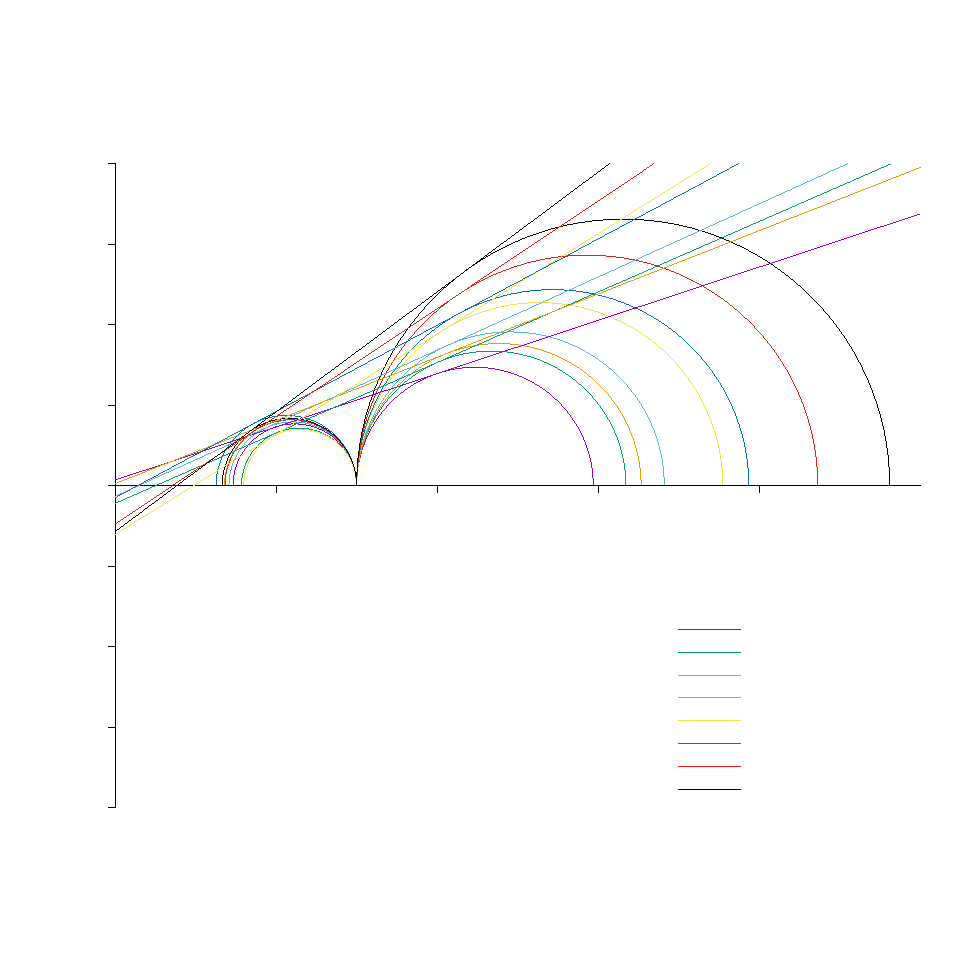
\includegraphics[width={453.50bp},height={453.50bp}]{./Cercle_1000_residuel}}%
    \gplfronttext
  \end{picture}%
\endgroup
}
                \caption{Cercles de Mohr}
            \end{figure}
        \end{column}
        \begin{column}{0.5\textwidth}
            \begin{figure}
                \centering
                \scalebox{0.5}{\input{mu_I_1000.tex}}
                \caption{$\mu(I)$ rhéologie}
            \end{figure}
        \end{column}
    \end{columns}
\end{frame}

\begin{frame}{3375 particules}
    \begin{columns}
        \begin{column}{0.5\textwidth}
            \begin{figure}[h]
                \centering
                \scalebox{0.4}{% GNUPLOT: LaTeX picture with Postscript
\begingroup
  \makeatletter
  \providecommand\color[2][]{%
    \GenericError{(gnuplot) \space\space\space\@spaces}{%
      Package color not loaded in conjunction with
      terminal option `colourtext'%
    }{See the gnuplot documentation for explanation.%
    }{Either use 'blacktext' in gnuplot or load the package
      color.sty in LaTeX.}%
    \renewcommand\color[2][]{}%
  }%
  \providecommand\includegraphics[2][]{%
    \GenericError{(gnuplot) \space\space\space\@spaces}{%
      Package graphicx or graphics not loaded%
    }{See the gnuplot documentation for explanation.%
    }{The gnuplot epslatex terminal needs graphicx.sty or graphics.sty.}%
    \renewcommand\includegraphics[2][]{}%
  }%
  \providecommand\rotatebox[2]{#2}%
  \@ifundefined{ifGPcolor}{%
    \newif\ifGPcolor
    \GPcolortrue
  }{}%
  \@ifundefined{ifGPblacktext}{%
    \newif\ifGPblacktext
    \GPblacktextfalse
  }{}%
  % define a \g@addto@macro without @ in the name:
  \let\gplgaddtomacro\g@addto@macro
  % define empty templates for all commands taking text:
  \gdef\gplbacktext{}%
  \gdef\gplfronttext{}%
  \makeatother
  \ifGPblacktext
    % no textcolor at all
    \def\colorrgb#1{}%
    \def\colorgray#1{}%
  \else
    % gray or color?
    \ifGPcolor
      \def\colorrgb#1{\color[rgb]{#1}}%
      \def\colorgray#1{\color[gray]{#1}}%
      \expandafter\def\csname LTw\endcsname{\color{white}}%
      \expandafter\def\csname LTb\endcsname{\color{black}}%
      \expandafter\def\csname LTa\endcsname{\color{black}}%
      \expandafter\def\csname LT0\endcsname{\color[rgb]{1,0,0}}%
      \expandafter\def\csname LT1\endcsname{\color[rgb]{0,1,0}}%
      \expandafter\def\csname LT2\endcsname{\color[rgb]{0,0,1}}%
      \expandafter\def\csname LT3\endcsname{\color[rgb]{1,0,1}}%
      \expandafter\def\csname LT4\endcsname{\color[rgb]{0,1,1}}%
      \expandafter\def\csname LT5\endcsname{\color[rgb]{1,1,0}}%
      \expandafter\def\csname LT6\endcsname{\color[rgb]{0,0,0}}%
      \expandafter\def\csname LT7\endcsname{\color[rgb]{1,0.3,0}}%
      \expandafter\def\csname LT8\endcsname{\color[rgb]{0.5,0.5,0.5}}%
    \else
      % gray
      \def\colorrgb#1{\color{black}}%
      \def\colorgray#1{\color[gray]{#1}}%
      \expandafter\def\csname LTw\endcsname{\color{white}}%
      \expandafter\def\csname LTb\endcsname{\color{black}}%
      \expandafter\def\csname LTa\endcsname{\color{black}}%
      \expandafter\def\csname LT0\endcsname{\color{black}}%
      \expandafter\def\csname LT1\endcsname{\color{black}}%
      \expandafter\def\csname LT2\endcsname{\color{black}}%
      \expandafter\def\csname LT3\endcsname{\color{black}}%
      \expandafter\def\csname LT4\endcsname{\color{black}}%
      \expandafter\def\csname LT5\endcsname{\color{black}}%
      \expandafter\def\csname LT6\endcsname{\color{black}}%
      \expandafter\def\csname LT7\endcsname{\color{black}}%
      \expandafter\def\csname LT8\endcsname{\color{black}}%
    \fi
  \fi
    \setlength{\unitlength}{0.0500bp}%
    \ifx\gptboxheight\undefined%
      \newlength{\gptboxheight}%
      \newlength{\gptboxwidth}%
      \newsavebox{\gptboxtext}%
    \fi%
    \setlength{\fboxrule}{0.5pt}%
    \setlength{\fboxsep}{1pt}%
    \definecolor{tbcol}{rgb}{1,1,1}%
\begin{picture}(9070.00,9070.00)%
    \gplgaddtomacro\gplbacktext{%
      \csname LTb\endcsname%%
      \put(814,1466){\makebox(0,0)[r]{\strut{}$-40$}}%
      \put(814,2239){\makebox(0,0)[r]{\strut{}$-30$}}%
      \put(814,3011){\makebox(0,0)[r]{\strut{}$-20$}}%
      \put(814,3784){\makebox(0,0)[r]{\strut{}$-10$}}%
      \put(814,4557){\makebox(0,0)[r]{\strut{}$0$}}%
      \put(814,5329){\makebox(0,0)[r]{\strut{}$10$}}%
      \put(814,6102){\makebox(0,0)[r]{\strut{}$20$}}%
      \put(814,6874){\makebox(0,0)[r]{\strut{}$30$}}%
      \put(814,7647){\makebox(0,0)[r]{\strut{}$40$}}%
      \put(946,4274){\makebox(0,0){\strut{} }}%
      \put(2491,4274){\makebox(0,0){\strut{}$20$}}%
      \put(4037,4274){\makebox(0,0){\strut{}$40$}}%
      \put(5582,4274){\makebox(0,0){\strut{}$60$}}%
      \put(7128,4274){\makebox(0,0){\strut{}$80$}}%
      \put(8673,4274){\makebox(0,0){\strut{}$100$}}%
    }%
    \gplgaddtomacro\gplfronttext{%
      \csname LTb\endcsname%%
      \put(209,4556){\rotatebox{-270}{\makebox(0,0){\strut{}$\tau$ (kPa)}}}%
      \put(8505,4656){\makebox(0,0){\strut{}$\sigma_n$ (kPa)}}%
      \csname LTb\endcsname%%
      \put(5698,2079){\makebox(0,0)[r]{\strut{}$I = 10^{-3}: \varphi = 18.99^{\circ}, c = 0.09$ kPa}}%
      \csname LTb\endcsname%%
      \put(5698,1859){\makebox(0,0)[r]{\strut{}$I = 10^{-2}: \varphi = 20.60^{\circ}, c = -0.15$ kPa}}%
      \csname LTb\endcsname%%
      \put(5698,1639){\makebox(0,0)[r]{\strut{}$I = 10^{-1}: \varphi = 30.64^{\circ}, c = -2.16$ kPa}}%
    }%
    \gplbacktext
    \put(0,0){\includegraphics[width={453.50bp},height={453.50bp}]{./Cercle_3000_residuel}}%
    \gplfronttext
  \end{picture}%
\endgroup
}
                \caption{Cercles de Mohr}
            \end{figure}
        \end{column}
        \begin{column}{0.5\textwidth}
            \begin{figure}[h]
                \centering
                \scalebox{0.5}{\input{mu_I_3000.tex}}
                \caption{$\mu(I)$ rhéologie}
            \end{figure}
        \end{column}
    \end{columns}
\end{frame}


\end{document}
